\documentclass{article}
\usepackage[utf8]{inputenc}

\title{Ordres multiplicatifs}
\author{Leonardo Saba}
\usepackage[french]{babel}
\usepackage[T1]{fontenc}
\usepackage{amsmath}
\usepackage{amssymb}
\usepackage{stmaryrd}
\usepackage{graphicx}

\begin{document}

\maketitle

\section{Introduction}
Soit $a\in\mathbb{N}$, $n\in\mathbb{N}^{*}$ et $m\in\mathbb{N}_{\geq 2}$, le but est de trouver pour quelles valeurs de n la congruence $a^n \equiv 1 [m]$ est vraie.\\
On peut remarquer que 0 est une solution triviale :
$a^0 = 1$ donc $a^0\equiv1[m]$ Soit $\alpha$ la première valeur possible non-nulle.
On remarque tout de suite que :\\
si $a^\alpha\equiv1[m]$\\
alors $(a^\alpha)^q\equiv1[m]$ $\forall q \in\mathbb{N}$\\
donc $a^{\alpha q}\equiv1[m]$ \\\\
Ainsi toutes les valeurs de n vérifiant cette congruence sont de la forme : $n=\alpha q$\\
On dira que $\alpha$ est l'ordre multiplicatif de a modulo m.

\section{Fonctions $f$ et $f^{-1}$}
La congruence présentée précédemment peut être posée d'une manière différente :\\
\begin{equation}
a^n\equiv1[m]\Leftrightarrow a^n = mq+1,\forall q \in\mathbb{N}\notag
\end{equation}

On peut en déduire n :\\
$n=\log_a(mq+1)$\\
$\Leftrightarrow n=\frac{\ln(mq+1)}{ln(a)}$\\
Soit $f(x)=\frac{\ln(mx+1)}{ln(a)}$ \\
Sa réciproque : $x=\frac{\ln(my+1)}{ln(a)}$\\
$\Leftrightarrow x\ln(a)=\ln(my+1)$\\
$\Leftrightarrow \ln(a^x)=\ln(my+1)$\\
$\Leftrightarrow a^x=my+1 \Leftrightarrow \frac{a^x-1}{m}=y$\\
Donc $f^{-1}(x)=\frac{a^x-1}{m}$

\section{Nombres premiers}
Soit S l'ensemble des solutions entières non-nulles $y=f^{-1}(x)$ avec $y\in\mathbb{N}$ et $x\in\mathbb{N}$, on peut remarquer que la valeur $S_0$ correspond à la valeur $\alpha$ décrite en introduction.\\
Soit g la fonction satisfaisant:\\
$\begin{array}{ccccc}
g & : & (\mathbb{N}, \mathbb{N}_{\geq 2}) & \to & \mathbb{N} \\
 & & a,m & \mapsto & \alpha \\
\end{array}$\\ où a est la base et m le modulo\\
Prenons par exemple $a=3$, faisons varier les valeurs de m. Voici les valeurs de g(a, m) pour $m\in\llbracket 2~;~10 \rrbracket$ :\\
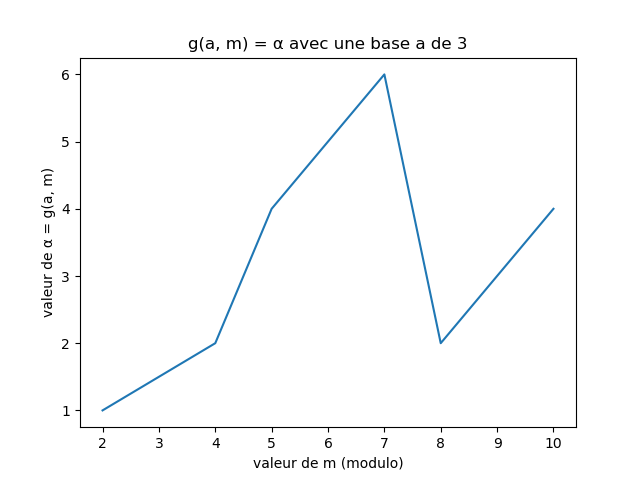
\includegraphics{images/Figure_1.png}\\
Les points ont été reliés pour une meilleure visibilité. Maintenant voyons les valeurs de $g(a,m)$ pour $m\in\llbracket 2~;~100 \rrbracket$ :\\
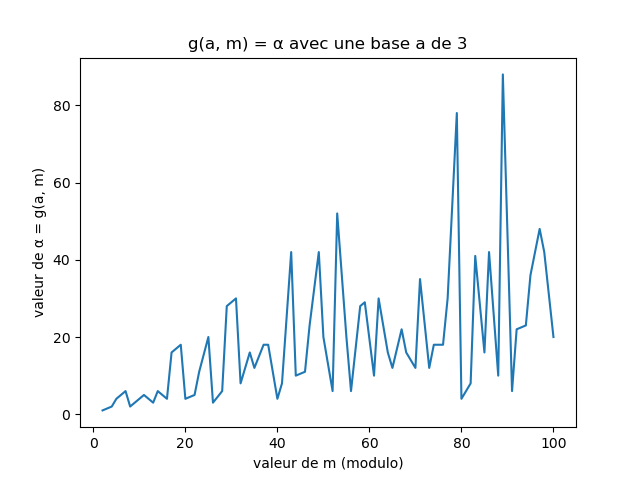
\includegraphics{images/Figure_2.png}\\
On peut remarquer des différents "pics" de la fonction, correspondant ici aux valeurs : 2, 5, 7, 17, 19, 29, 31, 43, 53, 79 et 89. Ces "pics" sont alignés sur la droite d'équation $y=m-1$. Ces valeurs semblent être des nombres premiers.\\
Ainsi les solutions $S_g$ de l'équation $g(a, m) = m - 1$ admettent $S_g\in\mathbb{E}$ avec parfois $\mathbb{E}\in\mathbb{P}$.
Cela peut se démontrer avec le petit théorème de Fermat.\\
Soit $p\in\mathbb{P}$ alors $a^{p-1}\equiv1[p]$ ainsi on retrouve la fonction $g(a, m)$ avec $m=p$ qui admet $g(a, p) = p - 1$ car ici $\alpha=p-1$. p est alors forcément solution de l'équation $g(a, m) = m - 1$ quand $m = p$. Donc m $\in\mathbb{E}$. Cependant, il est faux de dire que $\forall p \in\mathbb{P},p\in\mathbb{E}$ car la réciproque du petit théorème de Fermat n'est pas valable. En effet, $\mathbb{E}$ inclut aussi bien les nombres premiers que les nombres de Carmichael, qui sont des nombres absoluments pseudo-premiers.\\
Pour obtenir d'avantage de nombres satisfaisant cette équation, il est possible de faire l'union de différentes solutions en fonction des différentes valeurs de a.\\
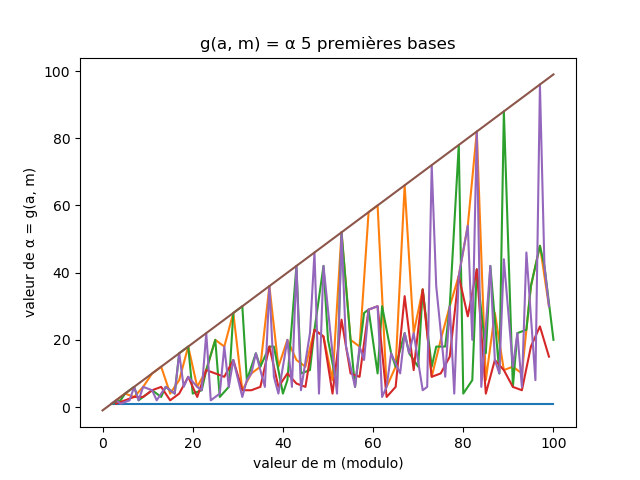
\includegraphics{images/Figure_3.png}\\
23 nombres premiers ou absolument pseudo-premiers ont été obtenus avec $a = 1$ jusqu'à $a=6$. La droite d'équation $y = m - 1$ a été représentée. On peut remarquer que la base $a=1$ admet toujours $\alpha = 1$. De plus la base $a=0$, n'a pas été mentionnée, celle ci n'admettant aucune solution.\\
Autrement dit, la valeur $\alpha$ vérifie cette équation :
\begin{equation}
\frac{a^{\alpha}-1}{m}-\left \lfloor\frac{a^{\alpha}-1}{m}\right\rfloor=0\notag
\end{equation}\\
De plus si l'on cherche une valeur telle que $\alpha\in\mathbb{E}$ alors on pose le système :
\begin{equation}
    \begin{cases}
      \frac{a^{\alpha}-1}{m}-\left \lfloor\frac{a^{\alpha}-1}{m}\right\rfloor=0\\
      \alpha = m - 1
    \end{cases}\notag
\end{equation}
En remplaçant $\alpha$ par $m-1$ :
\begin{equation}
\frac{a^{m-1}-1}{m}-\left \lfloor\frac{a^{m-1}-1}{m}\right\rfloor=0\notag
\Leftrightarrow Frac\left(\frac{a^{m-1}-1}{m}\right)=0
\end{equation}\\
Soit $h(m) = Frac\left(\frac{a^{m-1}-1}{m}\right)$ et $S_a$ l'ensemble de solutions de l'équation $h(m)=0$ en fonction d'une base a. Alors : \\
\begin{equation}
\forall p \in \mathbb{E}, p \in \bigcup_{n\in\mathbb{N}^{*}}S_n\notag
\end{equation}\\

\section{Approximation de la fonction $Frac$ par un polynôme trigonométrique}
La fonction $Frac$ utilisée précédemment dans la fonction h ainsi que ces généralités à n'importe quel modulo, trouvant ainsi l'ordre multiplicatif de a modulo m, se présente ainsi :\\
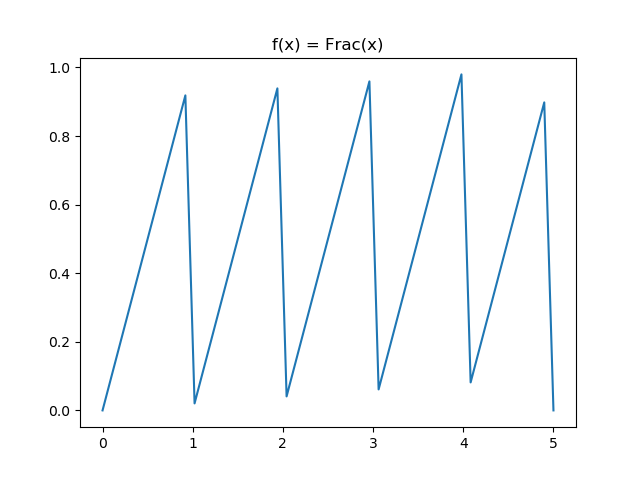
\includegraphics{images/Figure_4.png}\\
Cette fonction semble assez simple à approximer avec une série de Fourier car on remarque qu'il existe une fonction 1-périodique continue par morceaux admettant $f(t) = t$ sur l'intervalle $[0;1[$. On peut tout de suite indiquer que $\omega=\frac{2\pi}{1}=2\pi$. On peut ainsi calculer les coefficients : \\
\begin{equation}
\begin{split}
\alpha_0 & = \frac{1}{T}\int_{0}^{T}f(t)dt = \int_{0}^{1}tdt = \left[\frac{t^2}{2}\right]^1_0 =\frac{1^2}{2}-0=\frac{1}{2}\\\\\notag
\end{split}
\end{equation}
\begin{equation}
\begin{split}
\alpha_k & = \frac{2}{1}\int_{0}^{T}f(t)cos(k\omega t)dt\\
& = 2\int_{0}^{1}t\cos(k\omega t)dt\\
& = 2\left[\left[\frac{t\sin(k\omega t)}{k\omega}\right]^1_0 - \int_{0}^{1}\frac{\sin(k\omega t)}{k\omega}dt\right]\\
& = 2\left[\left(\frac{1.\sin(2k\pi)}{k\omega}-0\right) - \frac{1}{k\omega}\int_{0}^{1}\sin(k\omega t)dt\right]\\
& = 2\left[\left(\frac{\sin(2k\pi)}{k\omega}\right) - \frac{1}{k\omega}\left[\frac{\sin(k\omega t)}{k\omega}\right]^1_0\right]\\
& = 2\left[\left(\frac{0}{k\omega}\right) - \frac{1}{k\omega}\left(\frac{1.\sin(k\omega )}{k\omega}-0\right)\right]\\
& = 2\left[0-\frac{1}{k\omega}\left(\frac{\sin(2k\pi)}{k\omega}-0\right)\right]\\
& = 2\left[0-\frac{1}{k\omega}\frac{0}{k\omega}\right]=2\left[0-0\right]=0\\\\\notag
\end{split}
\end{equation}
\begin{equation}
\begin{split}
\beta_k & = \frac{2}{1}\int_{0}^{T}f(t)\sin(k\omega t)dt\\
& = 2\int_{0}^{1}t\sin(k\omega t)dt\\
& = 2\left[\left[\frac{-t\cos(k\omega t)}{k\omega}\right]^1_0 - \int_{0}^{1}\frac{-\cos(k\omega t)}{k\omega}dt\right]\\
& =2\left[\left(\frac{-\cos(2k\pi)}{k\omega}-0\right) - \frac{1}{k\omega}\int_{0}^{1}-\cos(k\omega t)dt\right]\\
& = 2\left[\frac{-1}{k\omega} - \frac{1}{k\omega}\left[\frac{-\sin(k\omega t)}{k\omega}\right]^1_0\right]\\
& =2\left[\frac{-1}{k\omega} - \frac{1}{k\omega}\left(\frac{-\sin(2k\pi)}{k\omega}-\frac{-\sin(0)}{k\omega}\right)\right]\\
& = 2\left[\frac{-1}{k\omega} - \frac{1}{k\omega}\left(\frac{-0}{k\omega}+0\right)\right]\\
& = 2\left[\frac{-1}{k\omega} - \frac{1}{k\omega}\times0\right]\\
& = 2\times\frac{-1}{k\omega}\\
& = \frac{-2}{k\omega} = \frac{-2}{2k\pi}=\frac{-1}{\pi k}\notag
\end{split}
\end{equation}\\\\
Ainsi avec ces coefficients on peut obtenir la série de Fourier suivante :
\begin{equation}
\begin{split}
S(x) & = \alpha_0 + \sum_{k=1}^{+\infty}\alpha_k\cos(k\omega x)+\beta_k\sin(k\omega x)
\\
& = \frac{1}{2}+\sum_{k=1}^{+\infty}0\times cos(2k\pi x)+\left(\frac{-1}{\pi k}\times sin(2k\pi x)\right)\\
& = \frac{1}{2}+\sum_{k=1}^{+\infty}\frac{-\sin(2k\pi x)}{\pi k}\\
& = \frac{1}{2}-\frac{1}{\pi}\sum_{k=1}^{+\infty}\frac{\sin(2k\pi x)}{k}\notag
\end{split}
\end{equation}\\
Par ailleurs, on peut facilement trouver une série de Fourier justifiant la fonction $f(x) = \left\lfloor x \right\rfloor$, en effet on a :
\begin{equation}
x = \left\lfloor x \right\rfloor + Frac(x) \Leftrightarrow \left\lfloor x \right\rfloor = x - Frac(x)\notag
\end{equation}\\
Soit donc la série de Fourier pour la fonction entière (floor) :\\
\begin{equation}
\begin{split}
\left\lfloor x \right\rfloor & = x - Frac(x)\\
\Leftrightarrow \left\lfloor x \right\rfloor & =  x-\left(\frac{1}{2}-\frac{1}{\pi}\sum_{k=1}^{+\infty}\frac{\sin(2k\pi x)}{k}\right)\\
\Leftrightarrow \left\lfloor x \right\rfloor & = x-\frac{1}{2}+\frac{1}{\pi}\sum_{k=1}^{+\infty}\frac{\sin(2k\pi x)}{k}\notag
\end{split}
\end{equation}\\

\section{Détermination réelle de l'ordre multiplicatif par un polynôme trigonométrique}

L'équation vérifiant $y=f^{-1}(x)$ avec $y\in\mathbb{N}$ et $x\in\mathbb{N}$ peut être désormais étendue à $\mathbb{R}$ par l'utilisation de polynômes trigonométriques des fonctions partie entière (floor) et partie décimale (frac).\\
On peut "forcer" $x$ à être entier, par l'utiliation de floor dans un premier temps :\\
\begin{equation}
y = f(\left\lfloor x \right\rfloor) \Leftrightarrow y = \frac{\ln(m\left\lfloor x \right\rfloor+1)}{\ln(a)}\notag
\end{equation}\\
Dans un second temps, sachant que $\forall x \in\mathbb{R}/ Frac(x)=0 \Leftrightarrow x\in\mathbb{N}$ :\\
\begin{equation}
Frac(y)=0 \Leftrightarrow Frac(f(\left\lfloor x \right\rfloor)) = 0 \Leftrightarrow Frac\left(\frac{\ln(m\left\lfloor x \right\rfloor+1)}{\ln(a)}\right)=0\notag
\end{equation}\\
Soit l'équation $E : Frac\left(\frac{\ln(m\left\lfloor x \right\rfloor+1)}{\ln(a)}\right)=0$, alors en remplaçant les différentes fonctions par leur polynôme trigonométrique associé on a donc :\\
\begin{equation}
E : \frac{1}{2}-\frac{1}{\pi}\sum_{k=1}^{+\infty}\frac{1}{k}\sin\left[\frac{2k\pi}{\ln(a)}\ln\left[m\left(x-\frac{1}{2}+\frac{1}{\pi}\sum_{k=1}^{+\infty}\frac{\sin(2k\pi x)}{k}\right)+1\right]\right]=0\notag
\end{equation}\\

Soit $T$ l'ensemble des solutions de $E$ en fonction d'une valeur de $a$ et de $m$, on peut déjà constater qu'une valeur $f(\alpha)$ obtenue, s'étend sur un intervalle de part la partie entière : $[f(\alpha) ; f(\alpha)+1[ \in T$, il faudra ainsi prendre la valeur minimum de cet intervale, ou prendre : $\forall x\in T, q\alpha = \left\lfloor x \right\rfloor \forall q\in\mathbb{N}$
Par ailleurs, par le même procédé, l'on peut obtenir une équation pour obtenir les élements de $\mathbb{E}$. Il suffit simplement de résoudre $h(\left\lfloor x \right\rfloor) = 0$. \emph{L'utilisation de "simplement" laisse à désirer.}\\
Par exemple, prenons pour $a=4$, $m=7$, ayant une précision (cela correspond au calcul d'une série partielle jusqu'à une borne maximale), ici \emph{1000}.
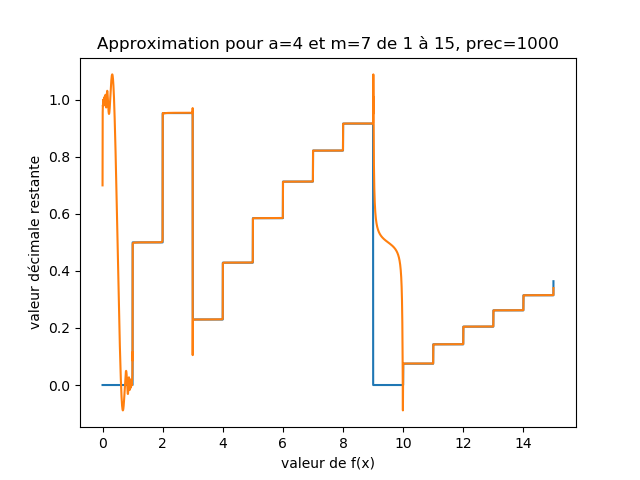
\includegraphics[scale=0.75]{images/Figure_5.png}\\
La courbe bleue correspond à la fonction utilisant la "vraie" fonction $floor$ et $frac$, celle en orange correspond à l'approximation.\\
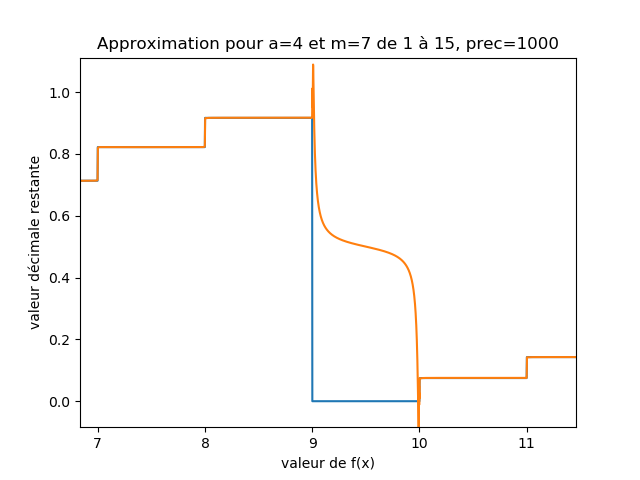
\includegraphics[scale=0.75]{images/Figure_6.png}\\
Cependant, l'on peut constater un décalage de la courbe orange par rapport à la véritable fonction. Ce décalage prend forme à toutes les valeurs où $E$ admet des solutions. Soit $S_1$ cette ensemble de solutions. On peut donc conjecturer que les véritables solutions de l'ensemble $S_2$ admettent $\forall s \in S_1, s - 1 \in S_2$.\\
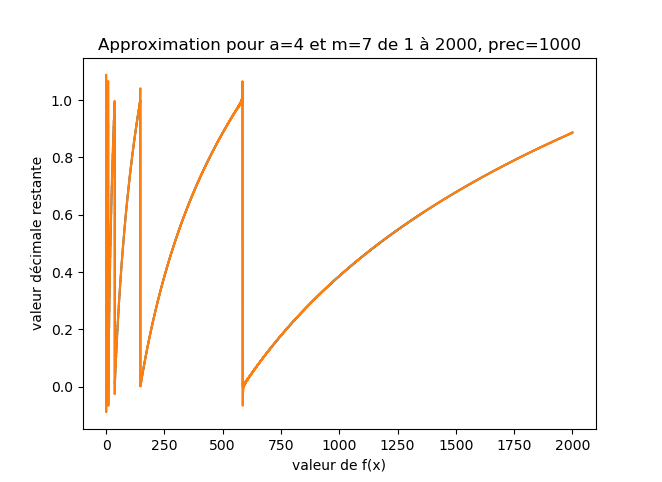
\includegraphics[scale=0.70]{images/Figure_7.png}\\
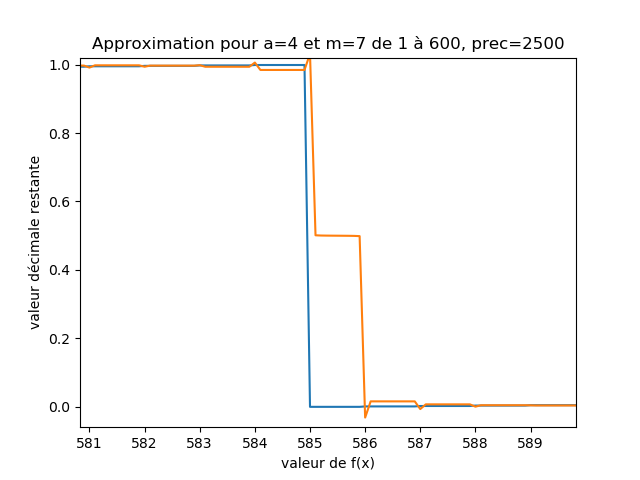
\includegraphics[scale=0.70]{images/Figure_8.png}\\
Une solution en $x=585$ existe, on remarque qu'elle apparaît en $x=586$ par l'approximation, toujours avec ce fameux décalage inexpliqué.

\section{Conclusion}
La détermination exacte par un calcul algébrique des valeurs $\alpha$ reste encore un long travail par la résolution de $E$ qui semble loin d'être triviale. La détermination des nombres premiers n'est pas abordée ici, par la réciproque fausse du petit théorème de Fermat. Cependant, serait-il possible d'avoir comme même une fonction de répartition des nombres premiers à travers l'ensemble $\mathbb{E}$ ? Aussi, la force de l'approximation peut laisser à désirer, de part le phénomène de Gibbs pouvant rendre les calculs faux, mais ce phénomène ne semble pas impacter grandement la validité des résultats. Enfin, comment expliquer le décalage de 1 des solutions de la fonction approximée, et surtout peut-on résoudre $E$ ?
\end{document}
